
\begin{figure*}[t]
    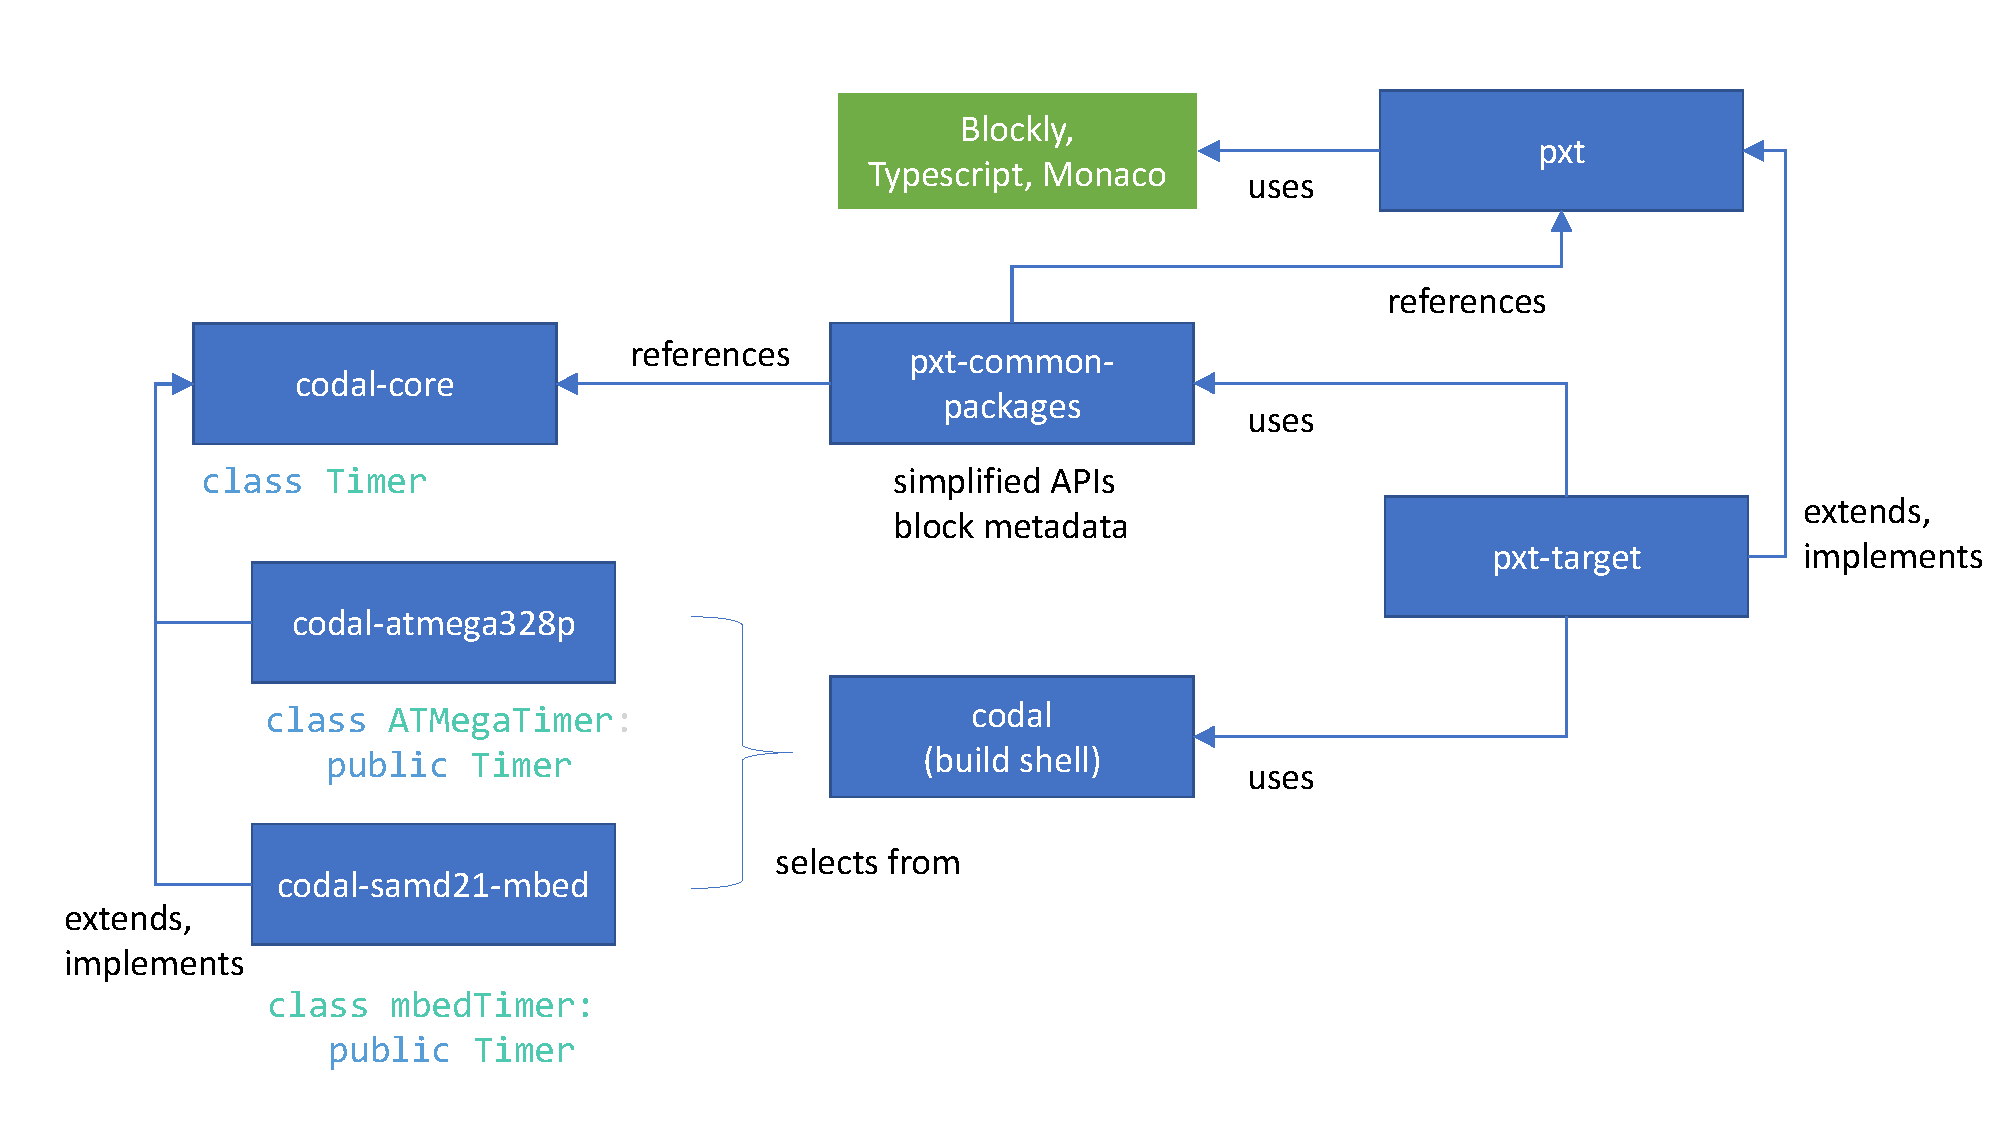
\includegraphics[width=5.5in]{reposFig.pdf}
    \caption{\label{fig:repos}Relationships between platform components/repos. Yellow boxes represent the \MC (PXT) components; blue
    boxes represent the \CO components; green boxes represent external components.}
  \end{figure*}
  

Figure~\ref{fig:repos} lists the major GitHub repos of the platform
and the dependences between them. Green boxes represent repos external to the platform
(note: not all repos are represented in the figure).

The \MC framework
is at \emph{\href{https://github.com/microsoft/pxt}{pxt}} (PXT is the previous codename of \MCN).
A \emph{pxt-target} extends the framework to create an environment for a specific board. Targets
for the three previously mentioned boards are at:
~\emph{\href{https://github.com/microsoft/pxt-microbit}{pxt-microbit}},
~\emph{\href{https://github.com/microsoft/pxt-adafruit}{pxt-adafruit}}, and
~\emph{\href{https://github.com/microsoft/pxt-arduino-uno}{pxt-arduino-uno}}.
The latter two targets make use of a common set of libraries,
\emph{\href{https://github.com/microsoft/pxt-common-packages}{pxt-common-packages}},
which build upon \CON's microcontroller independent core abstractions at
~\emph{\href{https://github.com/lancaster-university/\CO-core}{\COLN-core}}.

Platform- and microcontroller-dependent specialization and optimizations for
the SAMD21 and Atmega328 microcontrollers can be found at
~\emph{\href{https://github.com/lancaster-university/codal-samd21}{\COLN-samd21}},
and
~\emph{\href{https://github.com/lancaster-university/codal-atmega328p}{\COLN-atmega328p}}.
Not shown in the figure, the SAMD21 repo uses another repo for
MBED-specific optimizations for the Cortex-M0 processor: \emph{\href{https://github.com/lancaster-university/codal-mbed}{\COLN-mbed}}.

The repo \emph{\href{https://github.com/lancaster-university/codal}{\COLN}} provides the
tools for compiling a \CO target.  As can be seen in Figure~\ref{fig:repos},
\CO abstracts over platform and microcontroller specific
implementations, while PXT abstracts over programming editors and languages.
The \UF specification is at~\emph{\href{https://github.com/microsoft/uf2}{uf2}},
with implementations at~\emph{\href{https://github.com/microsoft/uf2-samd21}{uf2-samd21}}
and~\emph{\href{https://github.com/mmoskal/uf2-uno}{uf2-uno}}. These repos are not
shown in the Figure.
The pxt-microbit target uses a predecessor of the \CO called the DAL (at
~\emph{\href{https://github.com/lancaster-university/microbit-dal}{microbit-dal}}).
